\documentclass[sigconf]{acmart}

\usepackage{booktabs}
\usepackage{graphicx}
\usepackage{float}
\usepackage{pgfplots}

\setcopyright{rightsretained}

%opening
\title{An investigation into HTC performance of the Worldwide LHC Computing Grid}
\author{Jerrod T. Dixon}
\authornote{Graduate student at the Holland Computing Center}
\orcid{1234-5678-9012}
\affiliation{%
	\institution{University of Nebraska - Lincoln}
	\streetaddress{P.O. Box 1212}
	\city{Lincoln} 
	\state{Nebraska} 
	\postcode{43017-6221}
}
\email{jtdixon@cse.unl.edu}

\begin{document}

\maketitle

\begin{abstract}
The Worldwide LHC Computing Grid (WLCG) has been used to great effect to process the data produced at the Large Hadron Collider (LHC). 
\end{abstract}

\section{Introduction}
Implemented internationally, the Worldwide LHC Computing Grid (WLCG) operates as a conglomeration of computing centers managed by universities. The goal is to cooperate in processing the large amounts of data (~50 Petabytes in 2016 alone) produced by the Large Hadron Collider (LHC) at CERN.

Over the years, the processing methods have improved, and the implementation of the WLCG itself has grown in such a way that more data is produced than can be processed in a reasonable amount of time. This has resulted in backlogs of data requiring processing. Coordination of work is at issue as well, deciding when and where the transfer of the data to offsite locations should occur and where it is to go. 

Depending on which labs require the dataset, the data can be replicated in multiple geographically distant locations in such a way to allow easier access. Also, load balancing of work causes issues with users submitting work to be done to the same processing center. This can cause certain locations to become overloaded with requests for processing while others go almost unused. By extension the data also runs into the issue of being requested to do the calculations against getting called to a processing center that is not geographically close, for example the job is processed in Italy but the data exists in Spain, slowing the acquisition time. 

It has been an interesting subject but an investigation into how this work is done and split across sites has yet, to the authors knowledge, been done yet. For the purposes of this paper the data processed by the WLCG is investigated, with special attention paid to work done where the data for the job itself exists offsite from where the work is being done. Due to limitations of knowing how much data was pulled from where, only jobs with one data location are used.
\section{Background}
A grid network is classically defined as a software solution, implementing general commodity hardware, to enable the creation of a series of machines to achieve High Performance Computing (HTC). The benefit here, is that by implementing such a solution, allows for cheaper access to HTC style computing without requiring investment into designing and implementing specialized hardware to improve scientific computations.

In HTC solutions, following the previous definition, there are times when the cluster is not fully in use by the institution that developed it. Because of this, institutions across the globe have come up with methods to connect their personal clusters to a international grid. In this way, these HTC solutions are better utilized to achieve a higher usage saturation point, taking work from excessively busy systems and giving work to idle ones.
\subsection{HTCondor ClassAd data}
The data is gathered first using a python script to spider across the WLCG to pull ClassAd information about the work done on their respective clusters from the HTCondor\cite{condor} database. This data is then posted to an elasticsearch server to store for long term access. This gathers the statistics about the jobs themselves, just as duration of job, event rate, and efficiency of processing defined by the field \texttt{CpuEff} in Table \ref{tab:htcondor}. 
\subsection{MWT2 perfSONAR}
At the same time perfSONAR servers are setup at different regional locations to record different statistics about the network communications across links to other WLCG locations. This data includes throughput, packet loss, latency, and traceroute data (though for this investigation the traceroute data remains unused). This data is also posted to a MWT2 elasticsearch service at preset 'pulse' intervals.
\subsection{Important Fields}
In the HTCondor ClassAds there are a few fields in particular we are interested in, as can be seen in Table \ref{tab:htcondor}. There are however, CMS experiment specific values we are interested in as well, defined in Table \ref{tab:cmscondor}. Both of these sets of values are stored and reported by the HTCondor databases, recorded as ClassAds. On their own they can be interesting, but we are primarily concerned with their relation to networking information. Correlation will be the primary issue, as the perfSONAR data and HTCondor values are separate.
\begin{table}
	\caption{Typical HTCondor properties}
	\label{tab:htcondor}
	\begin{tabular}{ccl}
		\toprule
		Field &Description \\
		\midrule
		\texttt{CpuEff} & \parbox{4.5cm}{Percentage value of CPU time spent processing data over $X$ amount of time.} \\
		\midrule
		\texttt{JobCurrentStartDate}& \parbox{4.5cm}{Date and time the job started processing, not when it was submitted.} \\
		\midrule
		\texttt{JobFinishedHookDone}& \parbox{4.5cm}{Date and time the job finished processing, not when it left the system.} \\
		\midrule
		\texttt{WallClockHr}& \parbox{4.5cm}{Integer value of time spent processing, invariant of number of cores.} \\
		\midrule
		\texttt{RequestCpus}& \parbox{4.5cm}{Number of cores used in processing work.} \\
		\bottomrule
	\end{tabular}
\end{table}

\begin{table}
	\caption{CMS-specific HTCondor properties}
	\label{tab:cmscondor}
	\begin{tabular}{ccl}
		\toprule
		Field &Description \\
		\midrule
		\texttt{KEvents} & \parbox{4.5cm}{Number of events processed by the job in thousands.} \\
		\midrule
		\texttt{InputGB}& \parbox{4.5cm}{Size of input data for the job to process.} \\
		\midrule
		\texttt{ChirpCMSSWEventRate}& \parbox{4.5cm}{Clock rate of CPU as measured during the last 15 minutes of run time.} \\
		\midrule
		\texttt{Workflow}& \parbox{4.5cm}{Name of the workflow the job is working on in human readable format.} \\
		\bottomrule
	\end{tabular}
\end{table}
\section{Related Work}
The ability of this work to make investigations into the performance of jobs against network related data is directly related to the work of \cite{shawn}. As stated, the collaborations for the LHC rely heavily upon network technologies for the infrastructure but it is incredibly difficult to locate issues. It is from this inspiration that this work draws to investigate the work done utilizing the WLCG grid network while accounting for the affect network communications have on the processing and transference of data.

In addition, the primary gathering of HTCondor ClassAds is performed via a script designed and executed by \cite{brian}. Without this work there would be no easy method to investigate the HTCondor ClassAds distributed around the world, and read their values. In addition
\section{Experiment on CMS performance}
The data processed is gathered and interpreted from July 16th, 2016 to July 23rd, 2016.
\subsection{Relating Datasets}
These two datasets are unrelated beyond location data (that is, whether it was recorded at the 'source' location or the 'destination' location). What the network performance data records as 'source' and 'destination' is considered in the htcondor ClassAd data as 'processing location' and 'data location', respectively. To relate these two datasets, values stored in the MWT2 elasticsearch server are considered to be relevant if the 'source' location is the 'processing location' and the 'destination' location is the 'data location' where the dataset for the workflow to be processed is stored. In addition, the store date must be within the range of the processing time for the job itself. 

The relating data is stored on a staging elasticsearch server to hold the processed data. Each record in this third storage server relates to a ten minute period considering all work and network traffic during that period. Per a given 10 minute period values relating to the mean, median, min, max, and standard deviation ($\sigma$) of the distribution of each value considered is stored to maintain statistical qualities of the data the record represents.
\subsection{Processing}
Once this data is correlated it is stored, as previously stated, on a simplicial staging elasticsearch server. Graphs of these values are produced via python script, separating the graphs so that each is specific for a particular site, over individual links, on specific days, and per workflow. A line of best fit is calculated per value relationship. For interpreting this line of fit, the $r$ value is generally ignored as it is uncertain what a best fit $r$ value would be. The relationship we are primarily concerned with is if the slope of the line is positive or negative, to indicate an increasing or decreasing value. As such the p-value is used to determine of the line is valid results. Keeping with common practices, only lines with a value below 0.05 are observed.
\section{Results}
\begin{figure*}[!htb]
	\minipage{0.32\textwidth}
		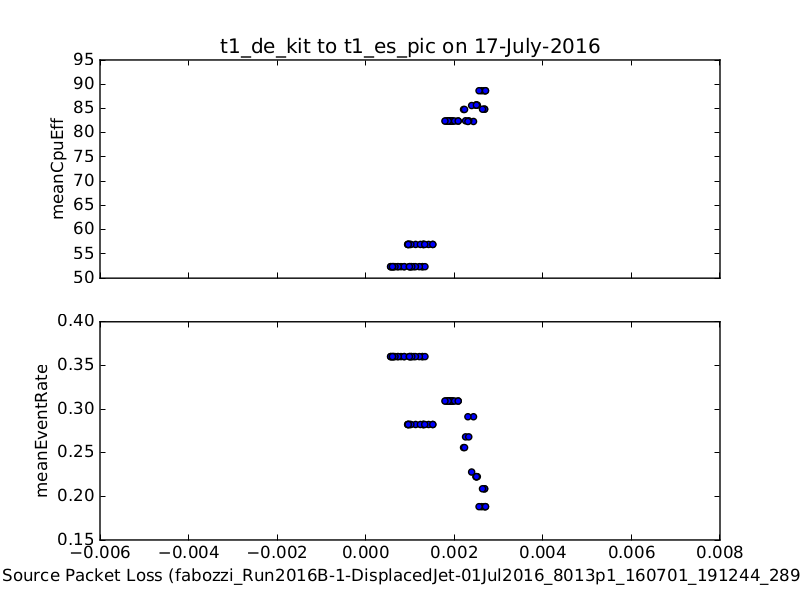
\includegraphics[width=\linewidth]{displacedjet_kit_pic}
		\caption{Packet Loss in workflow of DisplacedJet}
		\label{fig:displacedjet}
	\endminipage\hfill
	\minipage{0.32\textwidth}
		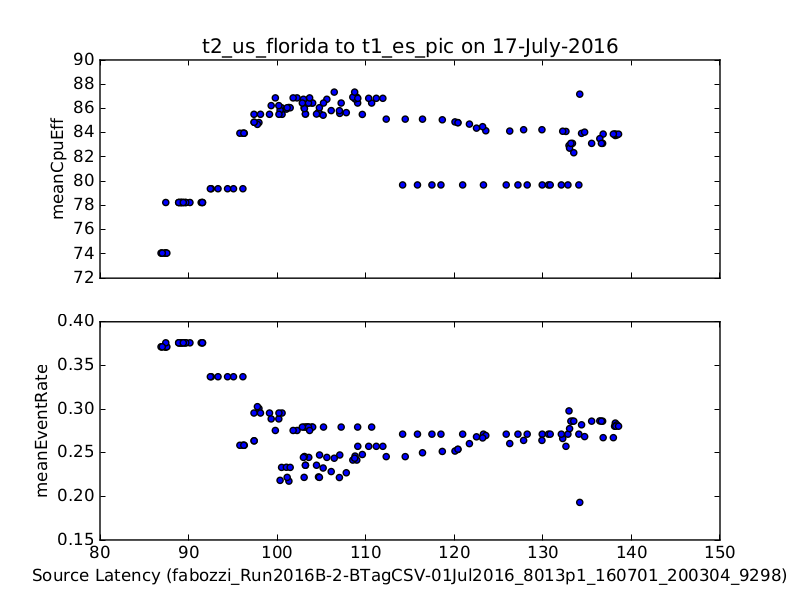
\includegraphics[width=\linewidth]{btagcsv_us_pic}
		\caption{Latency in workflow of BTagCSV}
		\label{fig:btagcsv}
	\endminipage\hfill
	\minipage{0.32\textwidth}
		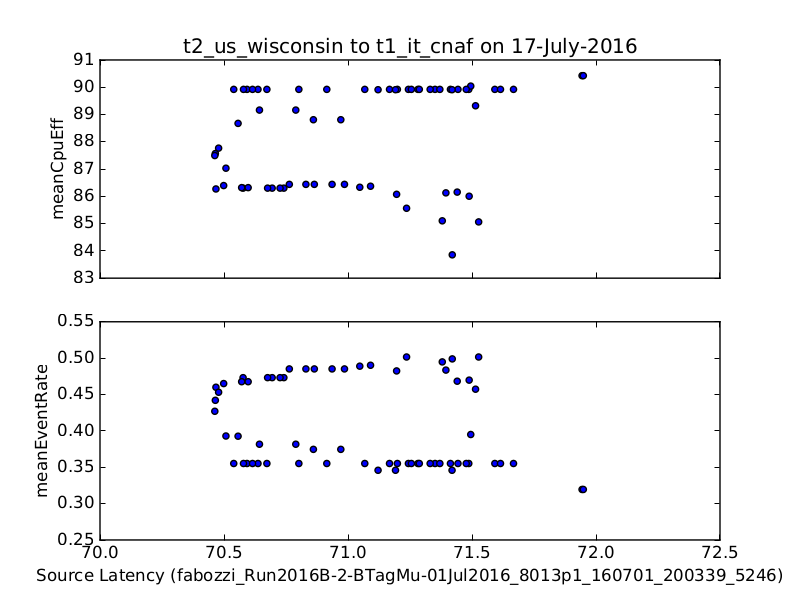
\includegraphics[width=\linewidth]{btagmu_us_cnaf}
		\caption{Latency in workflow of BTagMu}
		\label{fig:btagmu}
	\endminipage\hfill
\end{figure*}
\begin{table}
	\caption{Percent of time Workflows have inverse slopes with prefix fabozzi\_Run2016B}
	\label{tab:workflows}
	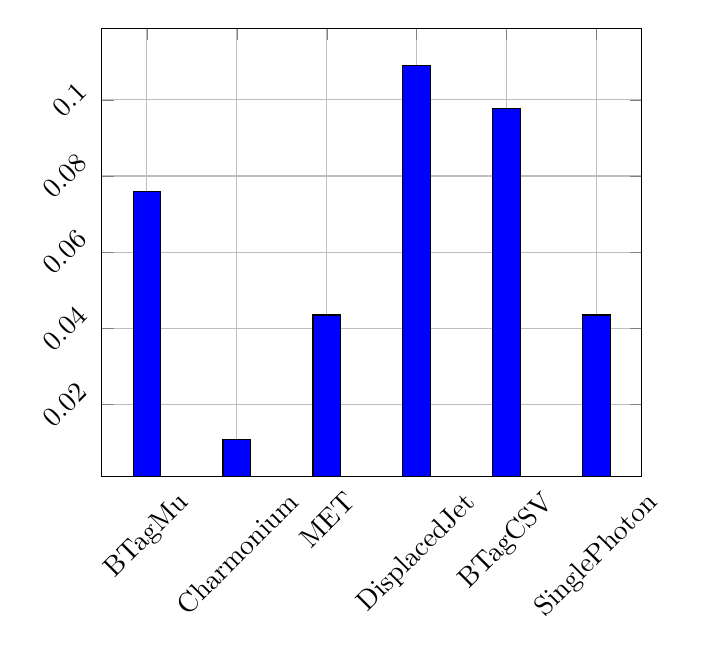
\begin{tikzpicture}
	\begin{axis}[
	symbolic x coords={BTagMu, Charmonium, MET, DisplacedJet, BTagCSV, SinglePhoton},
	xtick=data,
	x tick label style={
		grid=major,
		tick label style={rotate=45}
	},
	yticklabel style={/pgf/number format/fixed}
	]
	\addplot[ybar,fill=blue] coordinates {
		(BTagMu, .076)
		(Charmonium, .0109)
		(MET, .0435)
		(DisplacedJet, .109)
		(BTagCSV, .0978)
		(SinglePhoton, .0435)
	};
	\end{axis}
	\end{tikzpicture}
\end{table}
In the processing of data to calculate the relationships between HTCondor work data and perfSONAR networking data such as what is seen in Figure \ref{fig:displacedjet}, \ref{fig:btagmu}, and \ref{fig:btagcsv}, a line of linear regression is calculated for the relationship to best guess the quality of comparison. It is uncertain whether the r-value fitting the regression to the data is a valid comparison, so the calculated p-value is used to assume quality. The line of regression is not used to predict future values, only ensure the data is closely related. Since we are only curious about the relationship, whether both sets follow similar trends, we only need to know if the slope of the line follows a positive or a negative trend. As such, the p-value is assumed sufficient in qualifying the fit. Only relationships with a p-value that is less than 0.05 are accepted a valid set.

For the data collected, when comparing \texttt{EventRate} and \texttt{CpuEff} to networking information, 48.9\% of the time the two values have an inverse relationship. That is, while one improves the other declines. As seen in Table \ref{tab:workflows}, the distribution of which workflows show this relationship are displayed. 

It is uncertain what exactly is causing this relationship. Given the nature of work for the CMS experiment, a potential implication is the luminosity of the given data. For Scattering Theory, the concept of luminosity\cite{lumi} is the relationship between the number of events generated in the experiment over time. The field \texttt{KEvents} contains the number of events processed total, but there is no job data holding over how much time that number of events existed.
\section{Conclusion and future work}


\bibliographystyle{ACM-Reference-Format}
\bibliography{pearc} 

\end{document}
